\chapter{JavaScript}
Jedná se o objektově orientovaný skriptovací jazyk. V dnešní době je považován za jeden z nejvíce využívaných obecně používaných programovacích jazyků. Je nejvíce známý jako jazyk, který je součástí prohlížečů, ale je široce využíván v rámci webových serverů a aplikací\cite{ecmascript}. Používá se především pro tvorbu interaktivních webových stránek. JavaScript je především zpracováván na straně klienta v prohlížeči, ale je možné jej spustit také na straně serveru. JavaScript dodává webovým stránkám interaktivitu v podobě animací, pohyblivosti objektů, načítání dat bez potřeby obnovit stránku, validací vstupních hodnot a dalších funkcí. JavaScript je z tohoto důvodu používán ve více než 95 \% webových stránek \cite{historicaltrends}.

JavaScript byl vytvořen za účelem oživení statických webových stránek. Za vznikem tohoto programovacího jazyka stojí společnost Netscape\cite{ecmascript}, tedy tvůrci prvního grafického prohlížeče Mosaic. Netscape se nejprve pokoušel implementovat do jejich prohlížeče jazyk Java, který byl v té době velmi populární. Vývoj prohlížeče za použití tohoto jazyka byl ale neúspěšný, a tak bylo rozhodnuto o vytvoření nového programovacího jazyka. Společnost od Javy úplně upustila, ale za účelem zisku nově vyvíjený jazyk pojmenovala JavaScript. .Tento jazyk byl poté roku 1997 oficiálně vydán společností ECMA jako standard s názvem ECMAScript\cite{ecmascript}.
    \section{Principy a vlastnosti }
JavaScript je závislý na běhovém prostředí, přičemž tímto prostředím je nejčastěji webový prohlížeč. Toto prostředí poskytuje objekty a metody, se kterými mohou skripty interagovat, aby mohly prostředí upravovat (např. DOM webové stránky). Běhové prostředí také musí poskytovat možnost použití skriptů, v jazyce HTML se jedná o značku <script> \cite{eloquentjava}. 

JavaScript zpracovává veškeré zprávy po jednom a přebytečné zprávy ukládá do fronty. Následně JavaScript vyvolává funkce obsažené ve zprávě, vytváří rámec volání s argumenty funkce a lokálními proměnnými a obojí ukládá do zásobníku. Po dokončení funkce se zásobník volání zmenší. Když je zásobník volání po dokončení funkce prázdný, JavaScript přejde k další zprávě ve frontě. Tento proces se nazývá smyčka událostí. Zjednodušeně by se proces dal popsat frází „proveď do dokončení“ - každá zpráva totiž musí být zcela dokončena, než bude moci být zpracována další. Smyčka událostí je neblokující, vstup a výstup programu se tak provádí pomocí událostí a funkcí zpětného volání. Pro komplexnější výpočty spoléhá javascriptové jádro na web API, který zpracuje požadavek a až je dokončen, upozorní na sebe zpětným voláním. Jinými slovy JavaScript díky smyčce událostí a webovým API se zpětným voláním dokáže pracovat na více úkolech současně, jedná se tak o asynchronní provádění kódu. To například znamená, že JavaScript může zpracovat kliknutí myší, zatímco čeká na databázový dotaz, aby vrátil informace \cite{eloquentjava}.

Mezi vlastnosti odlišující JavaScript od řady jiných jazyků patří tzv. just-in-time kompilace. Pojmem se míní překládání programu do mezikódu těsně před provedením úkolu. JavaScript je dále vysokoúrovňovým jazykem, tedy jde o jazyk s vysokou abstrakcí instrukcí \cite{aboutjava}. Další vlastností je to, že je nenáročný na využití paměti a nezatěžuje příliš hardware. JavaScript je dále objektově orientovaný, což znamená, že objekty jsou asociativní pole s atributy. Objekty jsou často vytvářeny funkcí, která vytváři atributy objektu, přičemž tyto funkce se nazývají konstruktory. Tyto objekty mají své prototypy, podle kterých dědí vlastnosti, čímž se často vytváří řetězec prototypů. Další charakteristikou JavaScriptu je to, že je funkcionální. Funkce jsou v něm brány jako objekty, takže mohou obsahovat atributy a metody a mohou být anonymní - nemusí mít tedy jméno a mohou být používány jako parametry jiné funkce. Poslední vlastností, kterou zde chci zmínit, je dynamické typování, tedy to, že je typ proměnné určen pomocí hodnoty, kterou obsahuje. Funkce eval() je tak například schopná vyhodnotit řetězec znaků jako kód za běhu programu.

    \section{Technologie spojené s JavaScriptem}
S vývojem JavaScriptu vznikly také nové technologie založené na JavaScriptu, které výrazně ovlivnily aplikace na webu. Mezi nejpodstatnější patří JSON, AJAX, webové API, jQuery, Node.js, npm a TypeScript. Dále se mezi významné technologie spojené s JavaScriptem řadí aplikační rámce, kterým bude vzhledem k tématu této práce věnována samostatná kapitola.

        \subsection{JSON}
JavaScript Object Notation (JSON) je jak už název napovídá odvozen od objektových literálů v jazyce JavaScript. Jedná se o textový formát pro serializaci strukturovaných dat. Má velmi jednoduchá pravidla a používá základní typy a struktury, proto je možné jej používat v jakémkoli programovacím jazyce. Existují i další formáty, které by bylo možné k podobným účelům využít, ale při práci s JavaScriptem je nejpřirozenější uplatnit JSON, jelikož jiné formáty by s sebou nesly zbytečné komplikace, jako nutnost použití knihovny třetích stran a nebo imlementace vlastních převaděčů. S rostoucí popularitou JavaScriptu se JSON využíval v praxi čím dál častější a v současnosti je preferovaným a nejvyužívanějším textovým formátem.

JSON může reprezentovat čtyři základní datové typy - řetězce znaků (sekvence žádného nebo více znaků Unicode), čísla, Booleovské operátory ano/ne a prázdné hodnoty NULL. Dále obsahuje dva strukturované datové typy, tedy objekt a pole. Objekt je složen z dvojic sestávajcích z klíče a hodnoty, přičemž klíč je řetězec a hodnota může být řetězec, číslo, Booleovský operátor, NULL, objekt anebo pole. Pole je označení pro uspořádanou sekvenci s žádnou nebo více hodnotami. Objekt je uzavřen ve složených závorkách, mezi klíčem a hodnou musí být dvojtečka, páry se oddělují čárkou a pole jsou uzavřena v hranatých závorkách. Příkladem takového zápisu může být například kód zobrazený níže.

{"name":"John", "age":30, "car":null}

Generování a zpracování formátu JSON je velmi nenáročné, JSON totiž obsahuje pouze základní informace. Je pro programátora jednoduše čitelný a je snadné se jej naučit. Oproti formátu XML ale právě kvůli své jednoduchosti nemá podporu pro komplexní datové typy jako jsou obrázky a grafy. XML také dokáže vyobrazovat samotná data, protože se jedná současně i o značkovací jazyk \cite{introjson}.

        \subsection{AJAX}
AJAX je jedna ze zásadních technologií zlepšujících zkušenost uživatele při práci s webovou aplikací. Asynchronous JavaScript and XML neboli AJAX je soubor technologií pro modifikaci webové aplikace, získávání dat ze serveru a jejich prezentaci bez potřeby opakovaného načtení webové stránky. Před vznikem technologie AJAX musel server při znovunačtení webové aplikace, například e-mailové schránky, vždy sestavit celou stránku a znovu klientovi poslat veškerý kód v HTML, CSS a JavaScriptu společně s e-maily. Výše popsaný způsob komunikace byl velmi neefektivní a nadbytečně zatěžoval server a spojení s klientem. S využitím AJAX server zasílá pouze potřebné informace. Tento nový přístup ke zpracování informací na webu byl dalším krokem k webovým aplikacím, které se chovají jako nativní aplikace, tedy aplikace nainstalované v počítači. Hlavní technologií zakomponovanou v AJAX, která tuto plynulou komunikaci se serverem umožňuje, je XMLHttpRequest. Přestože se název odkazuje na formát XML, tato technologie může zažádat nejen o XML, ale i o jiné formáty dat (například již zmiňovaný JSON).Tato data se následně za pomocí manipulace DOM zobrazí na prezentační vrstvě aplikace. Může se přitom jednat o hodnoty z databáze anebo až celé struktury HTML a JavaScript kódu.\cite{ajax}

\FloatBarrier
\begin{figure}[!htb]
\label{AJAX}
\centering
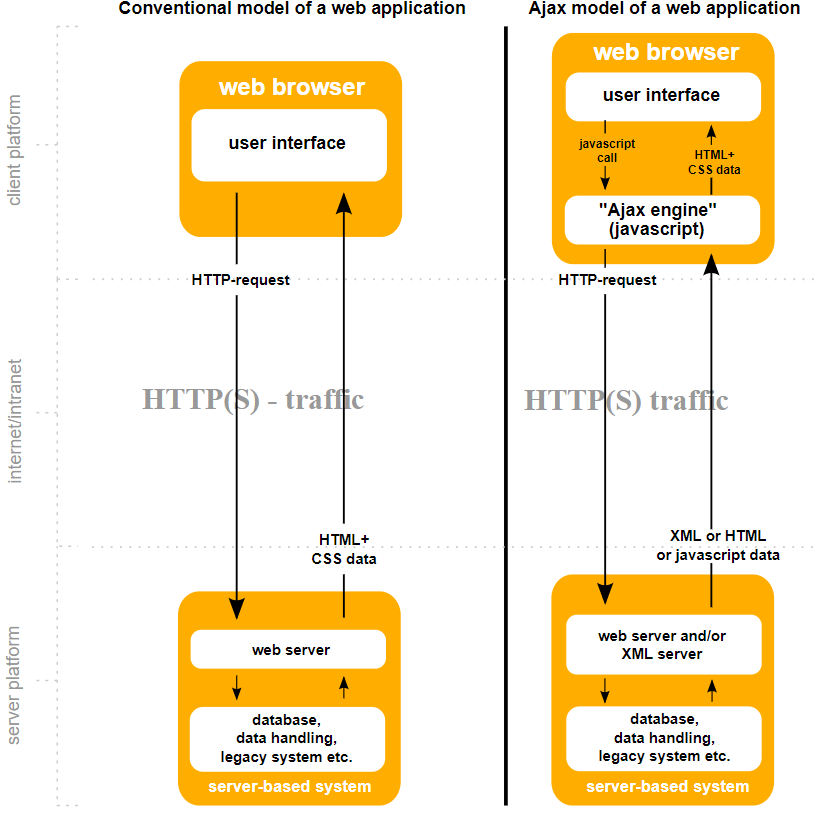
\includegraphics[width=\textwidth/2]{obrazky-figures/AJAX.png}
\caption{Konvenčí model pro webovou aplikaci versus aplikace používající AJAX.}
\end{figure}
\FloatBarrier

Na obrázku \ref{AJAX} je patrný rozdíl v komunikaci webové aplikace v konvenčním modelu ve srovnání s modelem používajícím AJAX. HTTP dotaz vytvoří přímo uživatel kliknutím, ale nejdříve je kontaktována AJAX logika běžící na pozadí pomocí JavaScriptu a teprve ta zašle HTTP dotaz. Jelikož není nutné čekat na získání odpovědi od serveru, je možné dále s webovou aplikací pracovat. V praxi ale uživatel získá odpověď téměř okamžitě.

        \subsection{Webové API}
Webové API (Application Programming interface) je rozhraní pro zpracovávání požadavků přes internet. Aplikace pošle požadavek, ten je následně zpracováván mimo aplikaci a po dokončení je aplikaci zasláno zpětné volání. Webové API mohou být AJAX dotazy na server nebo na databázi, může se jednat také o API prohlížeče jako je například odpočet času a podobně. Při zpětném volání je zaslán také objekt s odpovědí, a to nejčastěji ve formátech JSON a XML. API nepotřebují vědět, jaká aplikace je volá, potřebují znát pouze požadavek, který předají ve formátu definovaném v požadavku. Tento přístup je velmi podobný třídám s metodami v objektově orientovaném programování \cite{webapis}.
        \subsection{JQuery}
JQuery je volně dostupnou knihovnou, která zakomponovává více technologií, které zjednodušují práci s JavaScriptem. Známý slogan této knihovny, který ji současně i dobře vystihuje, je “Write less, do more” neboli “piš méně, udělej více”. Pro JavaScript zajistila jQuery zjednodušenou selekci a práci s DOM, DOM manipulaci pomocí CSS atributů a animace elementů a její součástí je také AJAX. Především tato knihovna ale zajišťuje kompatibilitu napříč prohlížeči. Každý prohlížeč zpracovával JavaScript vlastním způsobem, značné množství příkazů tak bylo nutné uzpůsobit pro prohlížeč, což byla jedna z největších kritik JavaScriptu. JQuery většinu s tím spojených problémů umí řešit, jelikož příkazy, které obsahuje, jsou vnitřně přeložené tak, aby jim prohlížeč rozuměl. Pro jQuery byla sepsána kvalitní dokumentace a stojí za ní velká komunita programátorů, zároveň se tato knihovna stala tak populární a revoluční, že je považována téměř za aplikační rámec.
Tabulka X. Srovnání zápisu základních příkazů v JavaScriptu a jQuery \cite{jquerybook}.

\FloatBarrier
\begin{table}[h!]
  \begin{left}
    \caption{Srovnání zápisu základních příkazů v JavaScriptu a jQuery}
    \label{tab:table1}
    \resizebox{\textwidth}{!}{
    \begin{tabular}{l|l}
      \textbf{JavaScript} & \textbf{jQuery}\\
      \hline
      document.querySelectorAll(‘.test-Class’) & \$(‘.test-Class’);\\\hline
      
      document.getElementById(‘#test-Id’).style.display = “none”; & \$(‘.test-Id’).hide();\\\hline
      
      \begin{tabular}{@{}l@{}}
      var h1 = document.CreateElement(“h1”); \\
      h1.innerHTML = “Nadpis”;\\
      document.getElementsByTagName(‘body’)[0].appendChild(h1);
      \end{tabular} & \$(‘body’).append(\$(“<h1/>”).html(“Nadpis”))\\\hline
      
      \begin{tabular}{@{}l@{}}
      var el= document.getElementById(‘test’);\\
      el.addEventListener('click', function() \{\\
      alert('TEST”');\\
      \}, false);
      \end{tabular} & 
      \begin{tabular}{@{}l@{}}
     \$(‘#test’).click(function() \{\\
      alert('TEST”');\\
      \});
      \end{tabular}\\\hline
     \end{tabular}}
  \end{left}
\end{table}
\FloatBarrier
Zápis v jQuery je oproti JavaScriptu zpravidla výrazně kratší a přehlednější (viz tabulku \ref{tab:table1}). Mnoho vlastností jQuery bylo postupem času integrováno do JavaScriptu. Podle W3Techs je jQuery používáno v 95 \% webových stránek používající JavaScript \cite{w3techs}.
        \subsection{Node.js}
Volně dostupné programovací prostředí (run-time) pro JavaScript s názvem Node.js umožňuje spouštět JavaScript mimo webový prohlížeč. Node.js byl postaven na Google V8 JavaScript jádře a byl navržen pro tvorbu škálovatelných síťových aplikací. Node.js obsahuje vestavěnou knihovnu, která umožňuje aplikacím fungovat jako webový server. Díky této technologii je možné používat JavaScript podobně jako jazyk PHP na serverové části aplikace. Node.js funguje na principu událostmi řízeném přístupu a v kombinaci s I/O API s neblokujícím přístupem, která optimalizuje přijímání a odesílání dat, umožňuje Node.js komunikaci mezi klienty a serverem v reálném čase. Node.js čeká na webovém portu na požadavky od uživatelů, po zachycení je požadavek vložen do jednovláknové smyčky událostí (event loop). Následuje zpracovávání požadavku, během něhož jsou zachytávány a zpracovávány další požadavky, které běží asynchronně na vlastních vláknech. Jednodušší požadavky tak mohou být zpracovávány rychleji.Celý proces zpracovávání požadavků je následující:
\begin{enumerate}
  \item Node.js získá požadavek od klienta.
  \item Požadavek je vložen do smyčky událostí, která je dále rozřazuje pro zpracování. Pokud příchozí požadavek není možné zpracovat, je vložen do fronty událostí.
  \item Požadavek je postupně zpracováván rozdělením na podúlohy. Pokud je možné úlohu zpracovat okamžitě nebo asynchronně(nebude tedy blokovat I/O), bude zpracována. Pokud se ale jedná o úlohu, která je synchronní, je předána některému z C++ vláken, které na něm dále pracují.
  \item Smyčka událostí je upozorněna dokončenou úlohou pomocí zpětného volání.
  \item Smyčka buď čeká na vyřízení jiné úlohy daného požadavku, nebo požadavek dokončí.
\end{enumerate}
Node.js exceluje při zpracovávání většího množství malých celků dat, tyto úlohy zpracovává s minimální odezvou \cite{nodejsevent}. Problém nastává pouze při provádění velkých výpočtů, které zaneprázdní všechna vlákna přidělená pro Node.js. V praxi je mnohem častější práce s malými výpočty, tudíž je tato nevýhoda velmi specifická a v kontrastu s výhodami je v běžném použití zanedbatelná. Jedná se také o relativně novou technologii, takže nativně podporuje moderní technologie jako například NoSQL databáze. Většina projektů vytvořených pomocí Node.js jsou zaindexované v registrech npm, tudíž se dají snadno dohledat a využít jako komponenty v aplikacích. Komunita spojená s Node.js se rychle rozrůstá, což podporuje zvyšování efektivity práce programátorů \cite{nodejsdevelopment}.

Společnosti jako jsou PayPal, Netflix, eBay převedly své webové aplikace na Node.js a zaznamenaly rychlejší vývoj aplikace, kratší vývojovou dobu a v některých případech menší počet lidí potřebných na vytvoření aplikace. Tato technologie také umožňuje snadné osvojení jazyka, JavaScript je totiž jeden z nejzákladnějších jazyků pro tvorbu na webu, a tak je přechod na serverovou logiku jednodušší. Komunikace mezi klientem a serverem probíhá ve stejném jazyku, což usnadňuje její přehlednost.

        \subsection{Npm}
Npm neboli Node Package Manager byl vytvořen pro správu balíčků k Node.js za účelem snadného sdílení, verzování a implementování kódu. Později se pak ale stal správcem všech javascriptových balíčků. V roce 2017 obsahoval 350 000 balíčků, čímž se stal největší kolekcí kódu v jednom jazyce. Npm se skládá z webové stránky, kterou lze využít pro objevování potřebných balíčků, Command Line Interface (CLI) neboli příkazového řádku, který běží v terminálu a umožňuje integrovat npm registr s obrovskou databází javascriptového softwaru a meta-informací s nimi spojenými. Základním úkolem balíčků je řešit konkrétní problémy nebo požadavky použitím cizího řešení tohoto problému. Často se přitom jedná o řešení osob kvalifikovanějších na danou problematiku. Balíčky by neměly řešit několik různých problémů naráz, ale měly by být definované pro specifickou potřebu. Díky tomu totiž vzníká modulární způsob programování, který podporuje systém vzájemného sdílení těchto modulů mezi programátory. Pokud nebude nalezeno potřebné řešení pro problematiku, může programátor implementovat vlastní a opět jej sdílet s ostatními. Balíčky mívají často podporu tvůrce či tvůrců a ostatní mohou navrhovat úpravy pro lepší implementaci. Idea nepsat kód, který už byl napsán mnohokrát předtím umožňuje rychlejší vývoj generických částí aplikace, jako je například přihlašovací formulář, navigace na stránce, tabulky apod. Tyto aplikační objekty je navíc možné převzít od předních a specializovaných vývojářů \cite{npmdocs}. 
        \subsection{TypeScript}
TypeScript je stručně řečeno rozšířenou verzí JavaScriptu. JavaScript totiž nikdy nebyl vytvořen k tomu, aby spravoval serverovou část aplikace, a proto mu chybí jisté prvky typické pro takové jazyky. Hlavní rozdílem je to, že JavaScript je čistě skriptovací jazyk. Dalším rozdílem je typování funkcí a proměnných, které podporuje strukturu kódu. TypeScript byl vytvořen, aby řešil právě tyto nedostatky. Jedná se o rozšíření jazyka JavaScript se zaměřením obohatit JavaScript o pravidla usnadňující programování aplikační logiky. TypeScript je silně typovaný, objektově orientovaný, kompilovaný jazyk. Kód v Typescriptu je při použití přeložen kompilátorem do čistého JavaScriptu. Jedná se tedy prakticky o maketu udržující strukturu kódu, která obsahuje několik prvků pro podporu vývoje kompletních webových aplikací. TypeScript je s JavaScriptem kompatibilní do takové míry, že pro konvertování javascriptového kódu do typescriptového stačí změnit koncovku souboru z .js na .ts. 

Díky podobnosti je veškerý kód JavaScriptu spustitelný v jazyce TypeScript, a tudíž i všechny knihovny JavaScriptu. TypeScript je navíc podporován na všech platformách, kde je spustitelný JavaScript - je tak podporována i veškerá infrastruktura a systém vzájemného sdílení kódu pomocí komponent či knihoven. Také run-time prostředí podporující JavaScript podporuje i typescript. Typescript navíc upozorňuje na chyby nalezené při kompilaci do JavaScriptu, což ulehčuje hledání chyb a jejich opravu \cite{typescriptweb}.

        \subsection{Webové komponenty}
Webové komponenty jsou sada technologií, které umožňují vytvářet vlastní znovupoužitelné webové prvky, které obsahují veškerou funkcionalitu zapouzdřenou a tím oddělenou od zbytku kódu. Tyto prvky je pak možné používat napříč aplikací bez vzniku konfliktů. Jedná se tedy správnou metodiku v rámci programování, která je aplikovatelná na celé aplikace. Webové komponenty se skládají ze tří technologií. Technologie vlastně vytvořených webových prvků, jedná se o rozhraní API JavaScriptu, které umožňuje definovat vlastní prvky a jejich chování. Další technologie je Shadow DOM, jedná se o několik API JavaScriptu pro připojení stínového stromu DOM k prvku. Tento DOM se vykresluje odděleně od hlavního stromu DOM aplikace. Dále se k prvku připojí ovládání zapouzdřených funkcí. Funkcionalita prvku je tedy naprosto oddělena od funkcionality aplikace ve které je prvek vložen. Poslední technologií jsou HTML šablony, šablony se značí <template> tyto umožňují psát šablony které nejsou zobrazené na stránce, ale pořád určují strukturu komponenty \cite{webcomponentsaction}.